% Autor: Kryštof Glos

\chapter*{Úvod}
Procedurálně vytvářený obsah v herním průmyslu je velmi důležitou součástí her už po několik let. Mnoho her postavených na tomto principu, se již prosadilo na trhu a stále více se uplatňuje. Náhodné vytváření obsahu se používá například na tvoření herních map, věcí v místnosti, skládání různých dopředu vytvořených místností tak aby vznikla jedinečná mapa. Takto implementované hry mají výhodu v opakované hratelnosti a nepředvídatelnosti.

Cílem této práce je návrh a vytvoření prototypu 2D hry, v herním enginu Unity, založené na procedurálním generování herního obsahu. Samotný generační algoritmus pracuje s Perlinovým šumem a výškovými mapami, ty slouží k vytvoření elevace různých bodů na mapě.

Inspirací na téma hry je počítačová hra RimWorld, která se řadí do her typu Colony-sim. Jedná se o žánr, ve kterém hráč ovládá skupinu lidí, kolonii, kterou se snaží, pomocí dobrého vedení, dovést k nějakému danému cíli. V navržené hře je úkolem hráče dostat kolonisty do stavu prosperity a mimo stav nouze o potravu a zdroje. Pohyb kolonistů využívá takzvané NavMesh agenty, kteří spolupracují s vytvořenou navigační sítí (NavMesh).

Vytváření mapy je stěžejní částí celé hry, určuje zdroje pro hráče a tudíž částečně i obtížnost celé hry. Ve hře se objevují nepřátelé, kteří mají jednoduchou umělou inteligenci a jsou jednou z překážek, se kterou se hráč musí během hry vypořádávat. Implementace generačních algoritmů, AI nepřátel a dalšího je popsána v kapitole \ref{implementace}.

Hra je implementována v herním enginu Unity, které je v dnešní době, jedním z nejvíce používaných vývojových nástrojů pro vývoj her. Mezi další oblíbená vývojová prostředí se řadí například, GameMaker, Unreal Engine, Godot. O vývoji v jednotlivých enginech pojednává kapitola \ref{engines}.

Po dokončení implementační části bylo zahájeno experimentování s herními systémy a následovné uživatelské testování. Průběh a výsledky této části práce jsou dále popsány v kapitole \ref{experiments}.

\chapter{Vytváření obsahu v herním světě} 
\label{theory}
Ve světě her jsou dvě možnosti jak přistupovat ke tvoření obsahu, jedním z těchto způsobů je tradiční nebo také \hyperref[traditional]{mechanické}, je jednodušší, vzhledem k tomu že není potřeba žádný algoritmus, ale pracnější. Další možností vytváření obsahu je pomocí metod implementující náhodné nebo také \hyperref[procedural]{procedurální generování obsahu}. 

Hry které mají pouze dvě dimenze se nazývají 2D (z anglického two dimensions). Je mnoho žánrů 2D her, RPG (role playing game) hry na hrdiny s příběhem, strategií, Co-op (kooperační) které jsou postavené na spolupráci více hráčů, survival (hry o přežití), colony-sim (z anglického colonization simulation) které mají simulovat kolonizaci ovládanou hráčem a tak dále. Tato bakalářská práce se zabývá hrou žánru colony-sim. Je mnoho způsobů jak vyvíjet takovou hru, nejčastěji se používají takzvané \hyperref[engines]{herní enginy}, které takové vyvíjení hry ulehčují a jsou na to stavěné.


\section{Způsoby generování obsahu}
V této části porovnáme mechanické generování obsahu s procedurálním, vysvětlíme co je lepší kdy použít a jaké známe metody pro procedurální generování. Následující tři body popisují faktory, které je třeba zvážit při rozhodování, zda bude využita nějaká procedurální metoda generování, nebo bude lepší použít manuální design úrovní a obsahu:
\begin{description}
	\item[Žánr tvořené hry] Při vývoji například takové hry z prvního pohledu (FPS) hry, u které záleží hlavně na ovládání a souboji hráče proti hráči, není třeba vytvářet mapy a další obsah procedurálně. Většinou stačí vytvořit například pouze jednu úroveň a v takovém případě není třeba používat procedurální generování. Při hrách, které závisí na okolí, surovinách a přežití kde každá okolnost nějak ovlivňuje hráče, už procedurální generování hraje větší roli. Zároveň pro vytváření obsahu jako je text, může být PG velmi obtížnou volbou, neboť v RPG hrách bývá textová část velmi důležitá a generování textu je stále dost obtížné
	\item[Opakovaná hratelnost] Některé hry jsou dělané tak, že čím déle hráč hraje stejnou úroveň (anglicky level), tím více se zlepšuje a je za to například odměňován je právě manuální tvoření úrovní lepší než procedurální. Naopak u jiných her, které mají úrovně procedurálně generované, většinou hráč danou úroveň zvládne, pokračuje na další a nepředpokládá se že se k ní bude ještě vracet.
	\item[Aspekt designu hry] Jestliže hra závisí z velké části na jedné úrovni s jejími mechanikami, vlastnostmi a obsahem, pak je lepší ji vytvářet mechanicky a doladit všechny vlastnosti a interakce s hráčem.
\end{description}


\subsection{Mechanické generování obsahu}
\label{traditional}
Mechanický typ generování je jedním z nejobvyklejších tvoření obsahu ve hrách. Používá se převážně v žánrech, jako je RPG (Role Play Game), RTS (Real Time Strategy) a další, ve kterých pozice objektů a struktura mapy hraje velkou roli a bez lidské tvorby by nebylo dosaženo potřebných výsledků. Toto tvoření lze interpretovat jako proces u něhož se návrhář za pomoci různých nástrojů, které postupně aplikuje, snaží dosáhnout požadovaného výsledku. Jde tedy o metodu ručního vytváření obsahu kde designér, nebo grafik navrhuje a postupně vytváří úroveň, či jinou část hry tak, aby vyhovovala potřebám, ať už se jedná o pozici stromu, nebo o to co hráči sděluji NPC.

Díky tomuto přístupu nehrozí nesrovnalosti ve výsledku, například se nemůže stát že určitá část mapy bude nedostupná, nebo úplně nesmyslná. Další výhodou je, že výsledek bude přesně takový jak byl naplánovaný, avšak takovéto tvoření je u větších her, kde je nutná opětovná hratelnost, velmi časově náročné.

\subsection{Procedurální generování obsahu}
Tento typ vytváření obsahu se používá ve více žánrech, ale asi nejznámější z hlediska generování map je Roguelike, kde každá nová hra má unikátní náhodnou mapu. Procedurální generování se ovšem nepoužívá pouze na generování map, ale také na vytváření objektů, jako jsou stromy, textury, animace, text a další. Procedurální generování obsahu není úplně to stejné, jako náhodné generování obsahu. Více do hloubky je tento typ modelování krajiny a textur rozebrán v kapitole \hyperref[procedural]{Procedurální generování}.

V zásadě je to proces obrácený jak u mechanického generování obsahu. Uživatel sice stále definuje různé nástroje, které jsou použity pro vytváření obsahu, ale nikoli pro své vlastní použití, ale naopak je vytváří pro algoritmus. Uživatel dále určuje pravidla podle kterých se generátor musí řídit tak, aby se dobral kýženého výsledku.

\begin{figure}[H]
	\centering
	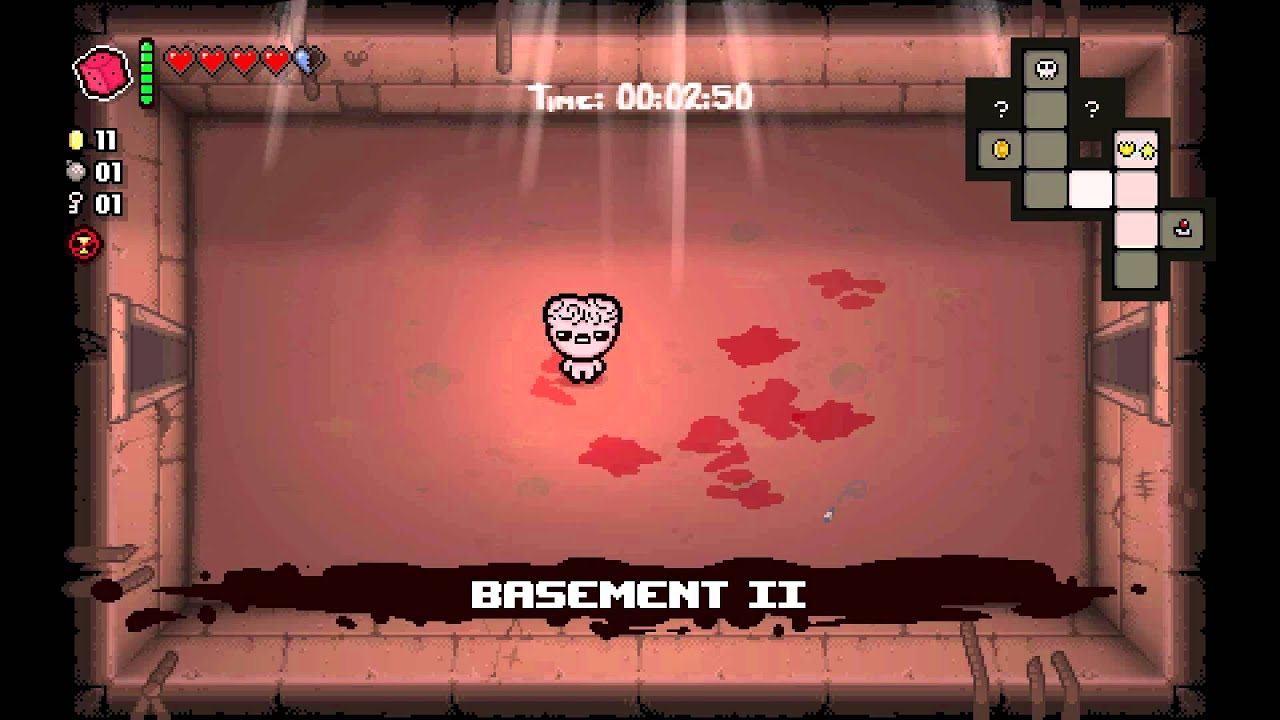
\includegraphics[scale=0.33]{obrazky-figures/BindingOfIsaac.jpg}
	\caption{Příklad hry Roguelike žánru jménem Binding of Isaac, vpravo nahoře je vidět mapa dungeonu, která je procedurálně vygenerovaná.}
\end{figure}

\subsubsection{Příklad procedurálního generování vegetace}
\label{proceduralExample}
Simulace lesních prostředí má mnoho aplikací, od zábavní po výzkumné modelování. Pro lepší představu uvádím příklad od Newlandse a Zaunera.~\cite{newlands2022procedural}

Program má funkci procedurálního generátoru lesů na mapě, cílem tohoto programu je náhodně naskládat stromy s rozumnými rozestupy od sebe. Metody pro vegetaci se dají opět řadit jako procedurální a mechanické. Neprocedurální přístup nabízí velkou kontrolu nad celým procesem a velký detail modelů, výměnou za cenu vyžadujícího značného množství uživatelských zásahů, často na úrovni vysazování rostliny po rostlině. V případě procedurálního generování, se jedná o modely které jsou zkonstruovány algoritmicky a kontrolovány skrze parametrické hodnoty, bez nutnosti vyšší úrovně manuálního vstupu nebo specializace v daném oboru.

Jednou z nejvíce prozkoumanou modelační technikou postavenou na rekurzivních hierarchiích je koncept \hyperref[lsystems]{L-systémů}. Existuje mnoho typů a rozšíření těchto systémů\cite{prusinkiewicz1986graphical}, včetně stochastických, parametrických, diferenciálních \cite{animationOfPlantDevelopment.}, citlivých na okolí \cite{syntheticTopiary}, nebo otevřených~\cite{PrusinkiewiczModelsOfPlants}.

Distribuce stromů na scéně lze udělat například pomocí simulace ekosystému. To vytváří více realistickou distribuci vegetace, než náhodné rozestavení, protože vznikají přirozená chování, jako je shlukování druhů a oblasti negativního růstu kolem stromů.~\cite{newlands2022procedural} Jedná se o simulace, ve kterých každá rostlina žije vlastní život, je ovlivňována ostatními rostlinami a vnějšími podmínkami.~\cite{Benes02ICCVG} 

Při Inicializaci simulace se pro každý specifický druh stromu vytvoří určité množství stromů (pro výpočet slouží rovnice~\ref{eq:treeCount}) ve věku $a_i\in\langle0,a_M\rangle$- kde $a_M$ je maximální věk stromu pro daný druh a jsou náhodně rozestavěny po oblasti od největšího po nejmenší.~\cite{newlands2022procedural}
\begin{equation}
\label{eq:treeCount} 
	n_I=\frac{d_0\cdot\rho}{n_T}w^2 
\end{equation}

Hodnota $n_I$ představuje počet instancí k vytvoření, $w$ je šířka scény, $d_0$ původní hustota pro objekt a $\rho$ je parametr hustoty jednotlivých objektů.

Po úspěšné inicializaci simulace běží $N$ kroků, kde $N_Y$ kroků utváří rok. Pro každý krok se děje následující:

\begin{itemize}
	\item[1] Pokud je konec roku, všechny stromy vysejí počet nových rostlin, v kruhu okolo nich.
	\item[2] U každého páru stromů je rostlina s menší důležitostí odstraněna.
	\item[3] Stromy starší než jejich maximální věk, jsou považovány za mrtvé a odstraněny.
	\item[4] Všechny rostliny rostou (jejich věk se zvýší o 1).
\end{itemize}


\begin{figure}[h]
	\centering
	\begin{subfigure}{0.475\textwidth}
		\centering
		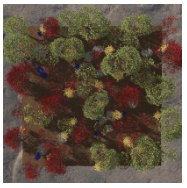
\includegraphics[scale=1]{obrazky-figures/treesStart.png}
		\caption{n=0}
	\end{subfigure}
	\begin{subfigure}{0.475\textwidth}
		\centering
		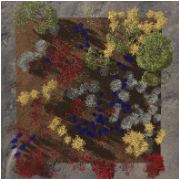
\includegraphics[scale=1]{obrazky-figures/treesEnd.png}
		\caption{n=1000}
	\end{subfigure}
	\caption[generatedTrees]{Vzhled ekosystému po inicializaci a rozložení vegetace po prvních 1000 iteracích. Je vidět že se vytváří shluky rostlinných druhů, tyto klastry zůstávají, pouze se mění jejich pozice.}
\end{figure}

\section{Procedurální generování v herním průmyslu}
\label{proceduralInGames}
Algoritmů na generování obsahu existuje mnoho, každý používá jiné nástroje, ale všechny se musí podrobovat pravidlům která stanovuje programátor a podle kterých se řídí. Je více způsobů a míst kde se dá procedurální generování uplatnit, různé způsoby a důvody jsou popsány v této kapitole.

\subsection{Text}
Skoro všechny hry používají text. Z důvodu že každá informace v textu musí odpovídat realitě, je nutno velké množství omezení pro generování. Například když je v textu informace že král je mrtvý \cite{liuDeep}, musí být toto tvrzení pravdivé.

Velkým plusem procedurálního generování textu je vyprávění \cite{madoc59000}, takto vytvořené příběhy jsou často kreativnější a zajímavější, než ty co by vytvořil člověk, neboť lidé mají sklony psát příběhy které již slyšeli, nebo ze svých zkušeností, což dost omezuje nápady.

\subsection{Krajina a úrovně}
Nejvíce obvyklý obsah který se ve hrách generuje, a který je zároveň hlavním zaměřením této práce, jsou krajiny a úrovně. Generování lokací, úrovní, nebo obsahu mapy lze jak u 2D her, tak u 3D her. Za úroveň nebo oblast lze označovat otevřené, třeba krajina s lesy, i uzavřené prostranství, vnitřek budovy, nebo jeskyně. Tato část PG je rozvedená a podrobněji popsaná v následující kapitole \ref{Krajina}.

\subsection{Textury}
Jednou z nejčastějších metod, která se používá na tvoření textur, jsou \hyperref[lsystems]{L-systémy}, nebo Perlinův šum, který je detailněji popsán v sekci \ref{noise}.

\subsection{Zvuky a hudba}
Většina her má soundtrack a zvukové efekty. Soundtrack obvykle nemá nijak zvlášť přísná pravidla, ale zvukové efekty musejí být výstižné a odpovídající akci v daný moment. 

Jukebox \cite{Dhariwal2020JukeboxAG} je model který dokáže generovat hudbu se zpěvem v originální nezpracované formě zvukových dat, s délkou v řádu minut, i s určením žánru a vokálního stylu. Modelů jako je tento již existuje více, avšak zatím to nejsou plně hodnotné soundtracky pro hry a ještě chvíli potrvá, než bude možné jednoduše vygenerovat hudbu a efekty pro hru pomocí pouhého nástroje.

\newpage

\chapter{Enginy na vývoj her}
\label{engines}
Herní engine představuje platformu složenou z interagujícího softwaru, který dohromady vytváří integrovaný celek a umožňuje spouštění samotných her. Herní engine se skládá z několika částí s přesně specifikovanou funkcionalitou: rendering, fyzika, síťování, zvuk atd.~\cite{nilson2007game} 

Platforem na vývoj her existuje mnoho, některými z nich jsou například Unity, Construct 2, MonoGame, Unreal Engine, nebo GameMaker Studio 2. Každý herní engine je v něčem jiný a tudíž se hodí na jiné žánry, nebo styly her. Při rozhodování, který engine použít, se z hlediska vývojáře musí zohlednit vícero faktorů, například podporovaný programovací jazyk, nebo platformu na kterou je hra vyvíjena.~\cite{vohera2021game}

\section{Construct 2}
Tento engine dovoluje lidem, kteří nejsou programátoři, vytvářet 2D hry. Používá drag and drop editor pro všechnu logiku založenou na událostech a chování. Může být rozšířen a skriptován pomocí JavaScriptu. 

I když Construct tvrdí že zveřejňují hry na většině mobilních a desktopových platformách, jejich primární cíl je HTML5/JavaScript. Tudíž jakákoliv verze která není ve vyhledávači je obsažena v DOM a obalovacím rozhraní umožňujícím použití JavaScriptu. Tato architektura obecně snižuje výkon.~\cite{engines}

\section{Unreal engine}
Podporuje multiplatformní vydávání her, jmenovitě DirectX, OpenGL, nebo WebGL. 

Jedná se o engine který je zdarma, ale pouze pro nekomerční užití a ve všech ostatních případech licencování softwaru za malé předplatné a licenční poplatek. Přes to, že původně byl vyvinut pro podporu \textit{Unreal} her z první osoby a neměl tolik nástrojů jako Unity, vyrostl Unreal Engine do podoby velmi výkonného enginu, schopného podporovat jakýkoli žánr her.~\cite{engines}

Skriptování je v enginu pomocí jazyka C++.

\section{Unity}
\label{unity}
Unity je multiplatformní herní engine, podporující vývoj her na Windows, Linux i macOS.
Vyvinula ho společnost Unity Technologies v roce 2005. Oproti jiným herním enginům podporuje vývoj her ve 2D, 3D, rozšířenou realitu (AR), nebo virtuální realitu (VR). 

Unity má více plánů které mohou vývojáři využívat, jedná se o personal, pro, enterprise a industry. Ze základu je pro všechny vývojáře zdarma k užívání, ale po překročení 100 000\$ za posledních dvanáct měsíců, je nutné pořídit si jeden z placených plánů. Tyto plány mají i jisté výhody, jako je třeba Havok Physics, přidávající robustní detekci kolizí a fyzikální simulace, technickou podporu, nebo prioritní frontu na zákaznickou podporu.~\cite{UnityPlans} 

Další výhodou je integrované fyzikální jádro PhysX, které pracuje v reálném čase a je vyvíjeno společností Nvidia. Toto jádro zahrnuje efektivní podporu pro multithreading a využívá akceleraci fyzikální simulace prostřednictvím GPU. Programování je v enginu zařízené pomocí jazyka C\#.

Z unity vzešlo mnoho oblíbených herních titulů, řadí se mezi ně hra ve virtuální realitě Beat Saber \ref{fig:beatSaber}, mobilní hra Pokémon Go \ref{fig:pogo}, nebo multiplatformní Cuphead~\ref{fig:cuphead}.
\begin{figure}[H]
	\centering
	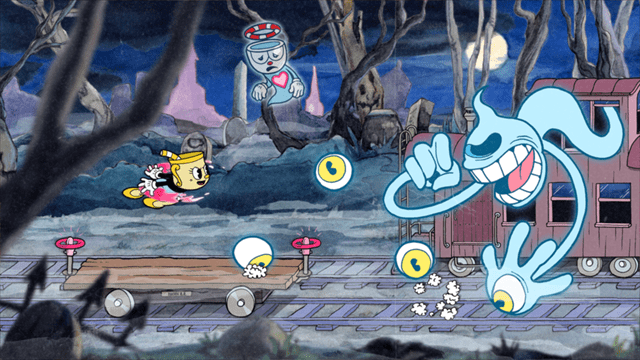
\includegraphics[scale=0.61]{obrazky-figures/Cuphead.png}
	\caption{Ukázka hry Cuphead}
	\label{fig:cuphead}
\end{figure}
\begin{figure}[H]
	\centering
	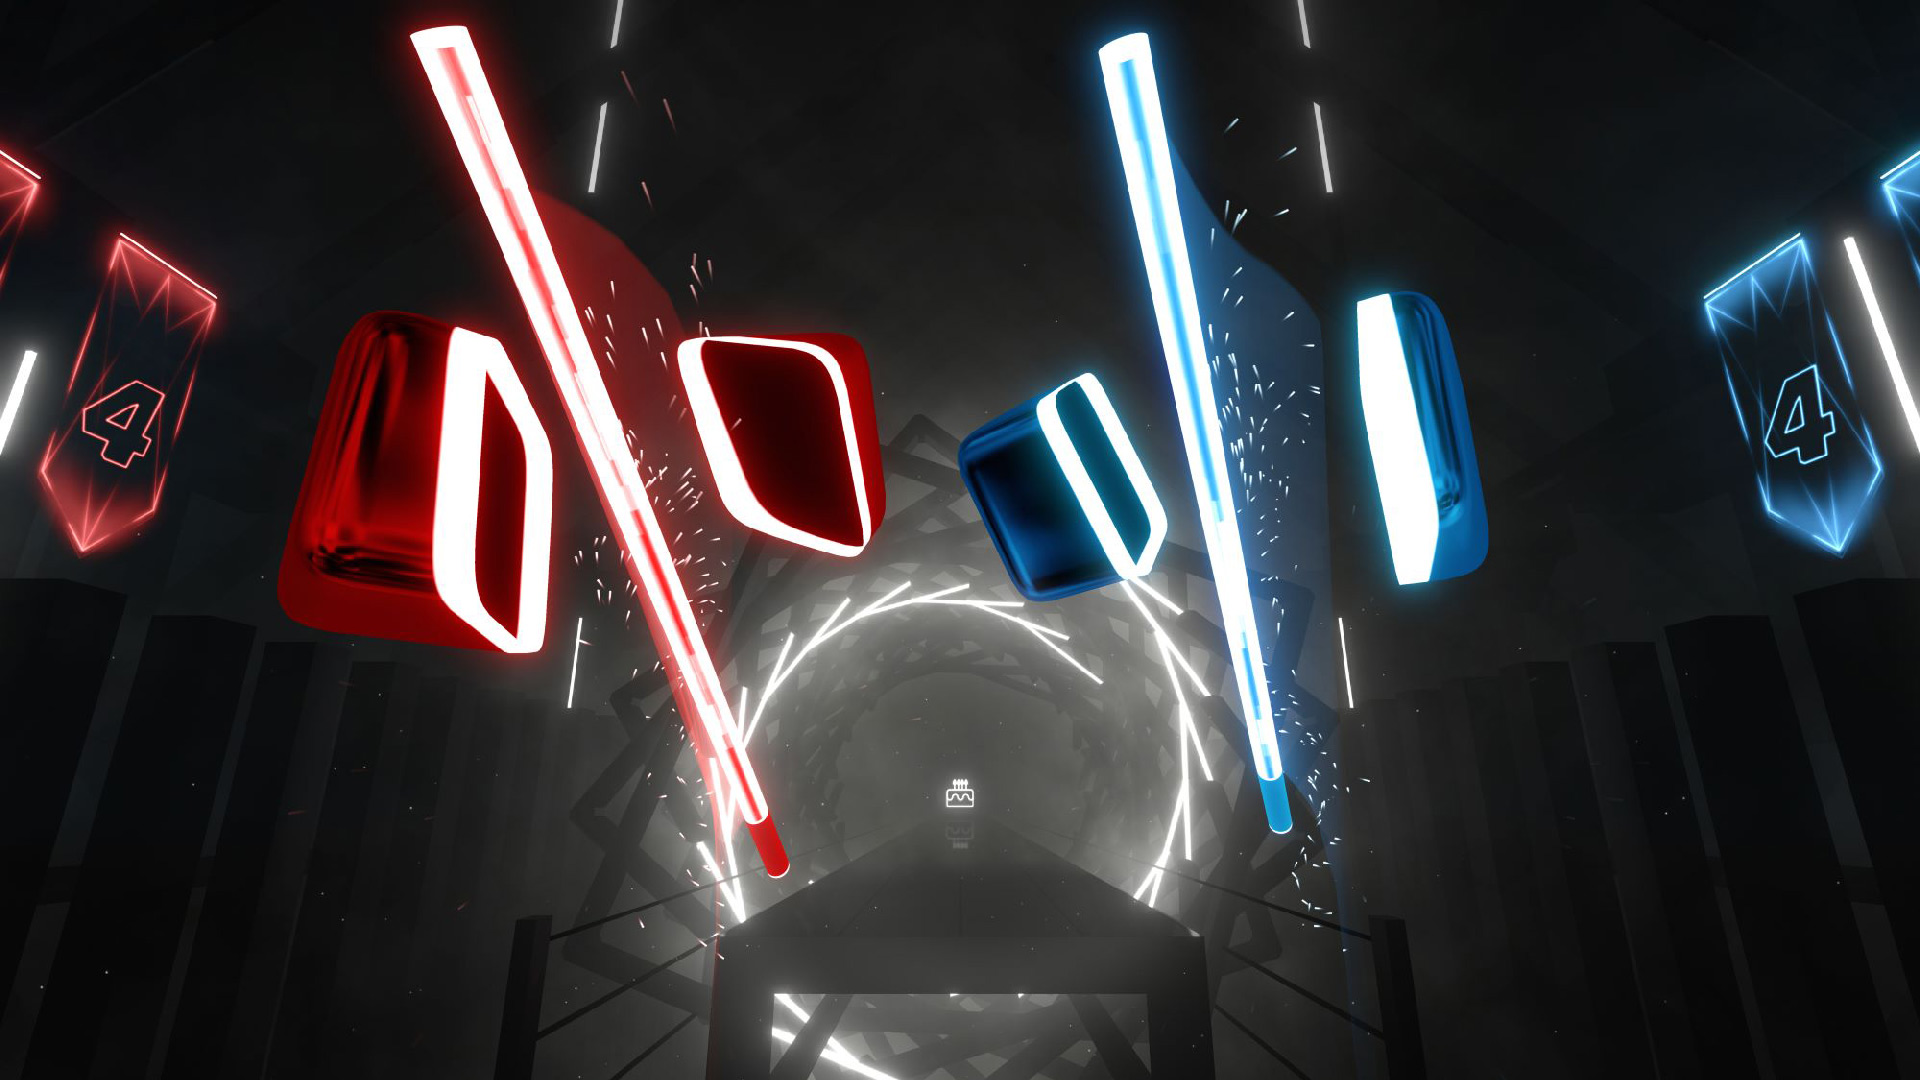
\includegraphics[scale=0.15]{obrazky-figures/BeatSaber.jpg}
	\caption{Ukázka hry Beat Saber}
	\label{fig:beatSaber}
\end{figure}
\begin{figure}[H]
	\centering
	
\includegraphics[scale=0.09]{obrazky-figures/PokemonGo.jpg}
	\caption{Ukázka mobilní hry Pokemon Go}
	\label{fig:pogo}
\end{figure}

\newpage

\chapter{Metody procedurálního generování}
\label{procedural}
Tato kapitola popisuje metody pro generování geometrie, vegetace, celulární automaty, perlinův šum a použití procedurálního generování v herním průmyslu, do detailu popisuje PG krajiny, generování fraktálů.

Procedurální modelování je téma které se aktivně zkoumá už přes čtyřicet let. Myšlenka je, jak již bylo zmíněno, aby obsah který se vytvářel ručně, dal modelovat pomocí navržené procedury automaticky. Takovýto přístup se již uplatnil na generování například textur, geometrických modelů, zvukových nahrávek, nebo animací. V roce 1980 se začalo pracovat s různými metodami na vytváření terénu, jako hory, pláně a jezera. Začal se také řešit růst rostlin a obecně práce s přírodou. \cite{inproceedings}

Roden and Parberry \cite{FromArtistry} pojmenovávají tento druh algoritmů \textit{amplifikační algoritmy (amplification algorithms)}, přijímají menší množství vstupních informací, které zpracují a vracejí větší objem dat na výstupu. Hendrikx et al. \cite{Hendrikx} pojímají procedurální generování jako alternativu k mechanickému navrhování obsahu, ale kladou důraz na zdokonalování a přidávání parametrů umožňujících zásah návrháře do takto vygenerovaných objektů.

\section{Celulární automaty pro procedurální generování}
\label{celular}
Celulární automaty se ve hrách používají intenzivně zejména pro modelování týkajícího se systémů v prostředí, jako jsou teplo, oheň, déšť, tlak a exploze. Zatím podle průzkumu nejsou známé žádné hry, které by postavili generování celého 2D herního světa, pouze pomocí celulárních automatů. Momentálně existují webové stránky, které možnost generování malých map pomocí mřížek navrhují, ale není jich mnoho a neexistuje žádné spolehlivé ohodnocení těchto algoritmů. \cite{articleCellular}

Původně byly CA vymyšleny Johnem Von Neumannem jako formální model sebereprodukujících se organismů. Šlo o dvou-dimenzionální celulární automat, kde každá buňka, tzv. cell, je malý čtverec na velkém čtverečkovaném papíru. Každá buňka má dva možné stavy, černý a červený, které jsou určeny jejich sousedstvím. V John Von Neumannově teorii, je sousedství tvořené čtyřmi přilehlými čtverci a na obrázku \ref{vonNeumann} jsou vyznačeny červenou barvou. \cite{Gong2017}

Nejznámější celulární automat byl vytvořen v roce 1970 britským matematikem Johnem Hortonem Conwayem, který se jmenoval Game Of Life. Stejně jako Von Neumannův byl i tento automat dvou-dimenzionální a mohli nabývat pouze hodnot živá, nebo mrtvá. Využívá Moorovo sousedství, které oproti Von Neumannově považuje za sousední buňky všech osm přilehlých, vyobrazené na obrázku \ref{moore}. Fungování automatu je následovné, buňka zůstává naživu, pokud má dvě, nebo tři sousedící buňky živé. Což simuluje, že buňka nepřežije pokud je osamělá, ale zároveň pokud je okolí přeplněné organismy, tak je utlačována. Další pravidlo je, že pokud je libovolná buňka mrtvá, může se "narodit", pokud jsou v sousedství alespoň tři živé buňky. Toto pravidlo má simulovat rození, kde každá buňka musí mít tři rodiče. Automat díky těmto jednoduchým pravidlům dokáže vytvářet simulace které působily jako živý organismus. \cite{Gong2017}

\begin{figure}[h]
	\centering
	\begin{subfigure}{0.475\textwidth}
		\centering
		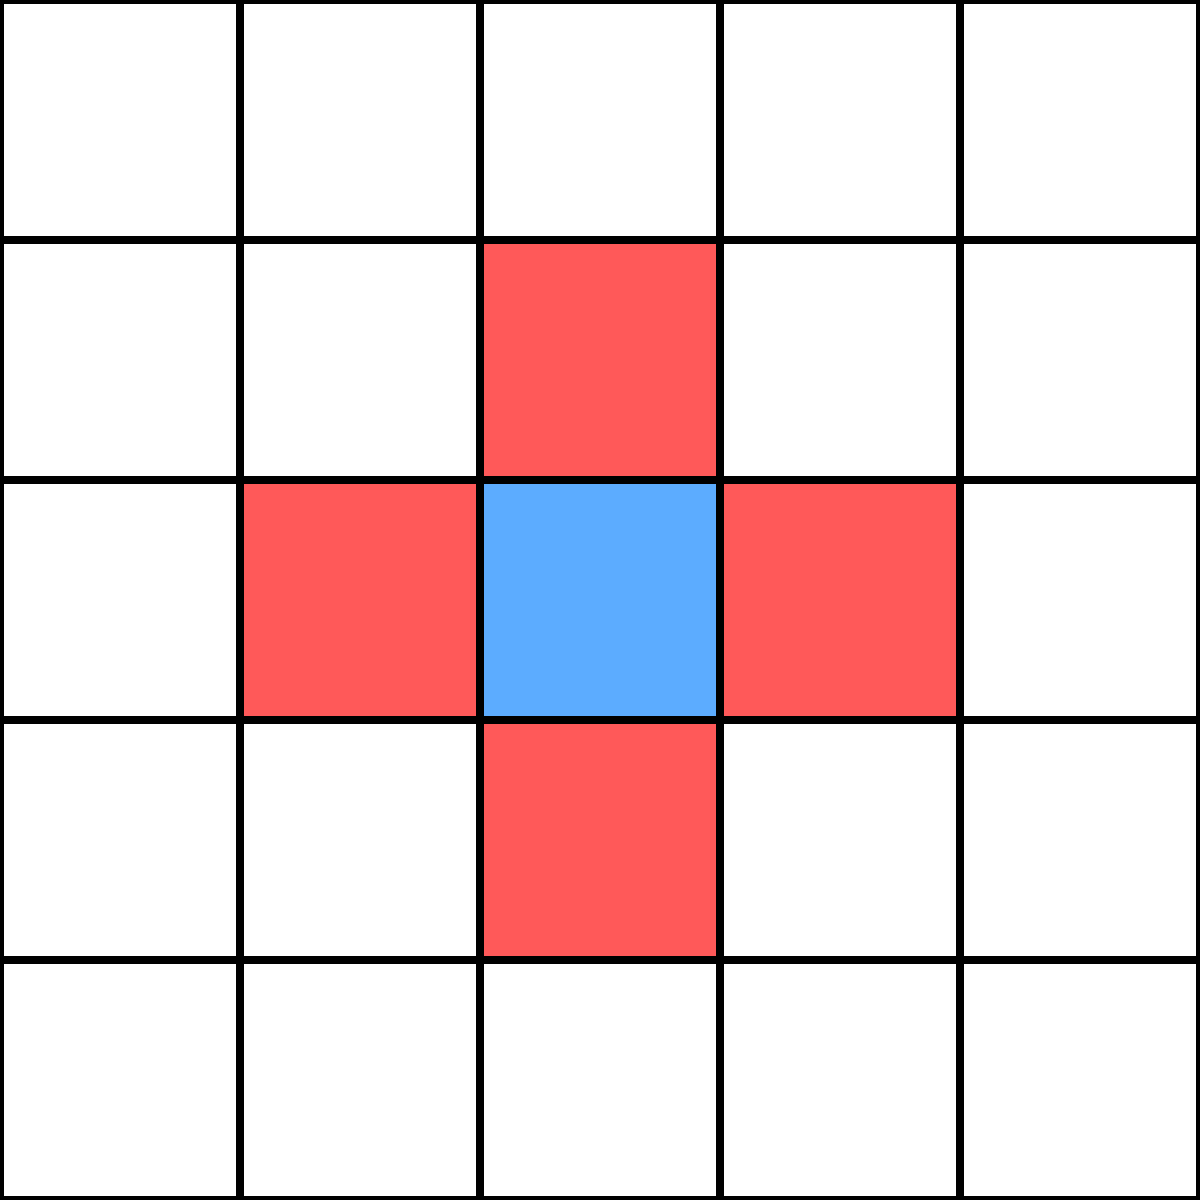
\includegraphics[scale=0.1]{obrazky-figures/Von_neumann_neighborhood.svg}
		\caption{Von Neumannovo sousedství}
		\label{vonNeumann}
	\end{subfigure}
	\begin{subfigure}{0.475\textwidth}
		\centering
		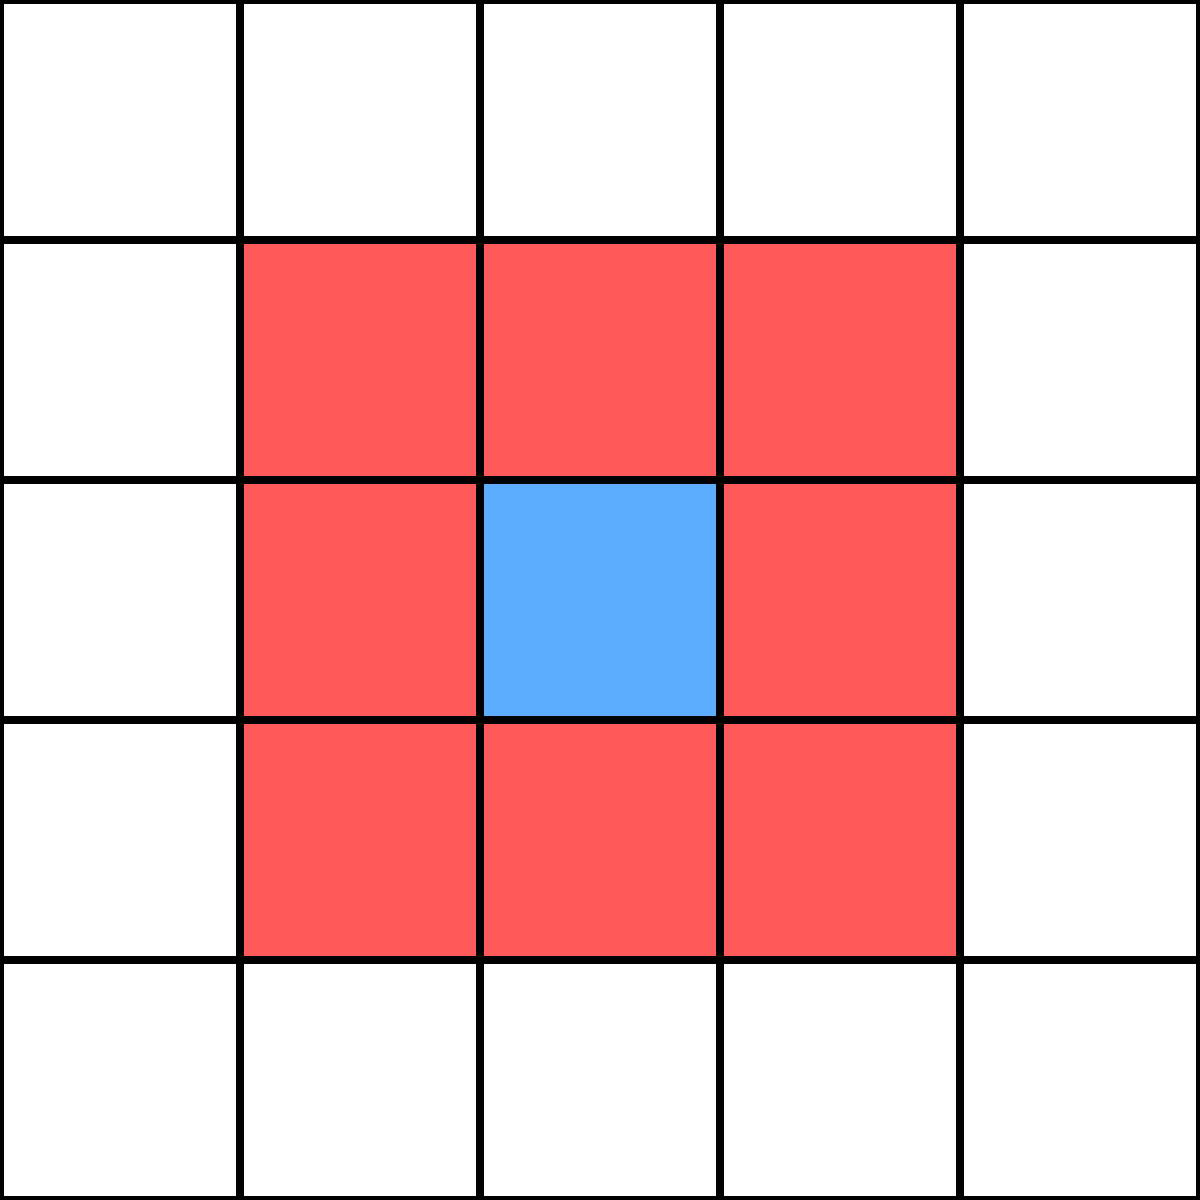
\includegraphics[scale=0.1]{obrazky-figures/Moore_neighborhood.svg}
		\caption{Moorovo sousedství}
		\label{moore}
	\end{subfigure}
	\caption{Sousedství z pohledu Von Neumanna a Moora}
\end{figure}

\section{L-systémy}
\label{lsystems}
L-systémy (Lindenmayerovy systémy) jsou formálním nástrojem \cite{prusinkiewicz1986graphical}, který se používá pro modelování vývoje rostlin a buněčných struktur. Tyto systémy byly zavedeny biologem Aristidem Lindenmayerem v roce 1968. \cite{inverseL-systems} Jedná se o paralelní řetězce přepisující systémy, za účelem modelovat růst celulárních organismů. L-systém $\mathcal{L}$ je entice

\[\mathcal{L} = \langle M,\omega,R\rangle ,\]


kde $M$ je abeceda L-systému, $\omega$ je axiom a $R$ je množina pravidel přepisování. Abeceda obsahuje parametrizované moduly $M = {A(P),B(P),\ldots}$, kde $P=p_1,p_2,\ldots,p_n$ jsou modulové parametry, jako jsou rotace, zvětšení, zmenšení.
Axiom $\omega \in M^+$ je neprázdná sekvence modulů a $M^+$ jsou všechny možné prázdné řetězce z $M$. Pravidla pro přepisování mají následující formu:

\[id_1:A(P):cond\rightarrow x,x \in M^*,\]
\[id_1:A(P):cond\rightarrow x,x \in M^*,\]
\[\ldots\]

kde $M^*$ jsou všechny možné řetězce z $M$ včetně prázdného $\epsilon$. Pravidlo $id_i$ přepisuje znak na levé straně z abecedy $A(P)$ posloupností písmen z pravé strany, pokud je podmínka $cond$ pravdivá. Modul, který se nenachází na levé straně pravidla, se nazývá \textit{terminální symbol}, neboť se nemůže dál měnit, všechny ostatní moduly se nazývají \textit{neterminální symboly}.\cite{prusinkiewicz2012algorithmic}

Každé písmeno má vlastní pravidlo derivace řetězce, ale probíhá paralelním provedením aplikovatelných pravidel, z množiny $R$ pro každé písmeno které obsahuje. Produkční pravidla přepisují začínající symbol sekvencí modulů a pokračují v úspěšných derivacích $\omega \Rightarrow m_1 \Rightarrow m_2 \Rightarrow \ldots,$ dokud není možné žádný další modul přepsat (řetězec končí pouze terminálními symboly), řetězec modulů je prázdný, kvůli aplikaci pravidla epsilon, nebo byl proces ukončen kvůli maximálnímu počtu iterací, které stanovil uživatel.\cite{lindenmayer1968mathematical}

Rekurze nastává v L-systémech tehdy, když se symbol z levé strany objevuje na pravé straně toho stejného pravidla (i když ne přímo). Nedeterminismus povoluje více pravidel pro jeden znak z abecedy. Toto navíc vyžaduje specifikaci pravděpodobnosti jejich aplikace.\cite{LINDENMAYER1968280}

\subsection{Geometrie pomocí L-systémů}
\label{lsystemGeometry}
Pro tvoření geometrie z textových řetězců, je každý řetězec reprezentován želvou, která vytváří geometrické symboly jako čáry, nebo dokonce 3D geometrii.
Ve 2D má želva stav $S(p,0)$ kde $p=[x,y]$ je její pozice a $0$ je směrový vektor, který udává směr jejího pohybu. 

Želva sekvenčně čte písmena interpretovaného řetězce z modulu od začátku po konec, kde každé písmeno je interpretované jako příkaz. Písmeno F si překládá jako "pohyb od $p$ směrem k $0$ o vzdálenosti d, která je zadaná a nakresli linku mezi starou pozicí a novou." Příkazy +($\alpha$) a $-(\alpha)$ mění směr pohybu želvy, jejím otočením doleva, či doprava o $\alpha$. Cokoliv v závorkách $[M^+]$ je geometricky interpretováno jako větev vygenerované struktury. Výhodou je že ne všechna písmena abecedy musí mít nastavenou geometrickou interpretaci, pokud ji nemají, tak je želva ignoruje.
\cite{prusinkiewicz1986graphical}

\begin{figure}[H]
	\centering
	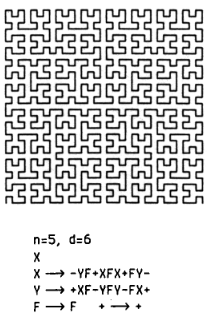
\includegraphics[scale=1]{obrazky-figures/L-system.png}
	\caption[L-system]{Vygenerovaných obrázek L-systémy želví interpretací, jsou zde vidět jednotlivé posuvy i hodnoty o které se posouvá}
\end{figure}
\newpage

\section{Šumy}
\label{noise}
Šumy se v počítačové grafice využívají například pro přidání kvalitních detailů do synteticky vytvořených obrázků. Perlinův šum, navržený Kenem Perlinem \cite{PerlinKen}, se v dnešní době používá ve vytváření procedurálních textur včetně mraků, vln, tornád, raketových cest, atd. Tato kapitola poskytuje detailní přehled jednotlivých funkcí generujících šum. Rozděluje tyto funkce do tří kategorií: gradientní mřížkové šumy \ref{LatticeNoises}, explicitní šumy \ref{ExplicitNoises} a řídké konvoluční šumy \ref{SparseNoises}. V každé z těchto kapitol je popsáno několik reprezentativních šumových funkcí rozebraných do detailu a další související příklady \cite{Lagae10}. 

\subsection{Definice šumu}
Šum je generátor náhodných čísel počítačové grafiky. \cite{PerlinKen} Jedná se o náhodný a neuspořádaný vzor, který je užitečný všude tam, kde je potřebný detail bez evidentní struktury. Jednoduchý šum pracuje například takto:
\begin{enumerate}
	\item Uvažujme množinu všech bodů v prostoru, jejichž souřadnice x, y a z jsou všechny celočíselné. Tuto množinu nazveme celočíselná mřížka. Každému bodu v této mřížce přiřaďte pseudonáhodnou hodnotu a gradientní hodnoty x, y a z. Přesněji, zobrazte každou uspořádanou posloupnost tří celých čísel do nekorelované uspořádané posloupnosti čtyř reálných čísel: $[a,b,c,d] = H([x,y,z])$, kde $[a,b,c,d]$ definují lineární rovnici s gradientem [a,b,c] a hodnotou d v bodě $[x,y,z]$. H 0 je nejlépe implementováno jako hashovací funkce.
	\item Pokud $[x,y,z]$ je na celočíselné mřížce, definujeme $Noise([x,y,z]) = d_{[x,y,z]}$. Pokud $[x,y,z]$ není v celočíselné mřížce, spočítáme hladkou (např. kubickou polynomickou) interpolaci mezi koeficienty rovnic mřížky, aplikovanou nejprve v x(podél hran mřížky), pak v y(ve vnitřních plochách mřížky z) a nakonec v z. Poté vyhodnotíme tuto interpolovanou rovnici v bodě [x,y,z]. 
\end{enumerate}

Ohodnocením hodnot takového šumu jsme schopni vytvářet jednoduché náhodné textury povrchu. \cite{PerlinKen} 

Například při ohodnocení šumu pouze bílou barvou:

\[color = white * Noise(point)\]

Výše uvedená textura má omezený frekvenční charakter, není zde žádný detail mimo určitý rozsah velikosti. Vzniklý obrázek je \ref{SpottedDoughnut}.

S hodnotou vrácenou funkcí Noise() \cite{Perlin2002ImprovingN} lze dále dělat mnoho různých věcí, s pomocí funkční kompozice, lze například mapovat různé rozsahy hodnot do různých barev:

\[color = Colorful(Noise(k * point))\]

V příkladu výše, byla textura škálovaná pomocí násobení domény funkce Noise() konstantou k. Jednou z výhod přístupu funkční kompozice je jednoduchost se kterou lze takovéto úpravy provádět, výsledný obrázek je níže \ref{ColoredDoughnut}.

\begin{figure}[H]
	\centering
	\begin{subfigure}{0.5\textwidth}
		\centering
		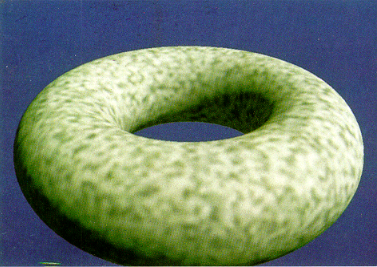
\includegraphics[scale=0.475]{obrazky-figures/SpottedDoughnut.png}
		\caption{Kobliha s puntíkovým vzorem}
		\label{SpottedDoughnut}
	\end{subfigure}
	\begin{subfigure}{0.4\textwidth}
		\centering
		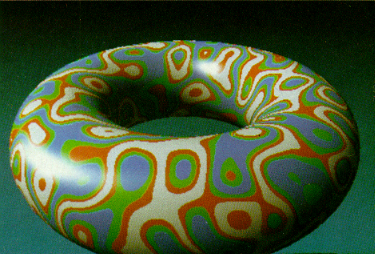
\includegraphics[scale=0.5]{obrazky-figures/ColoredDoughnut.png}
		\caption{Kobliha s barevným vzorem}
		\label{ColoredDoughnut}
	\end{subfigure}
	\caption{Na obrázcích jsou vidět koblihy se vzory podle aplikovaných ohodnocení šumů, obrázky jsou převzaty z \cite{PerlinKen}}
	\label{Doughnuts}
\end{figure}

\subsection{Gradientní mřížkové šumy}
\label{LatticeNoises}
\textit{Gradientní mřížkové šumy} vytvářejí šum pomocí interpolace, nebo konvolucí náhodných hodnot a/nebo gradientů definovaných v bodech celočíselné mřížky. Reprezentativním příkladem je \hyperref[perlinNoise]{Perlinův šum} \cite{Lagae10}.

\subsubsection{Perlinův šum}
\label{perlinNoise}
Roku 1985 Perlin představil \textit{Perlinův šum}, jeho slavnou procedurální funkci pro generování šumu.~\cite{PerlinKen}~\cite{Perlin2002ImprovingN} Perlinův šum určuje šum v bodě prostoru výpočtem pseudonáhodného gradientu u každého z osmi nejbližších vrcholů na celočíselné krychlové mřížce a následným provedením spline interpolace. Pseudonáhodný gradient je získán hashováním mřížkového bodu a použitím výsledku k výběru gradientu. Mřížkové body jsou hashovány pomocí postupné aplikace pseudonáhodné permutace na souřadnice k dekorelaci indexů do pole pseudonáhodných jednotkových gradientových vektorů. Sada gradientů se skládá z 12 vektorů definovaných směry od středu krychle k jejím hranám. Interpolantem je kvintický polynom, který zajišťuje spojitou derivaci šumu, neboli hladké přechody mezi jednotlivými body.

Již od svého uvedení před skoro čtyřmi desetiletími se Perlinův šum široce využívá v grafice, například při generování textur, které je vidět na obrázku \ref{PerlinVase}. Perlinův šum je rychlý, jednoduchý a nadále zůstává pilířem průmyslu.

\begin{figure}[H]
	\centering
	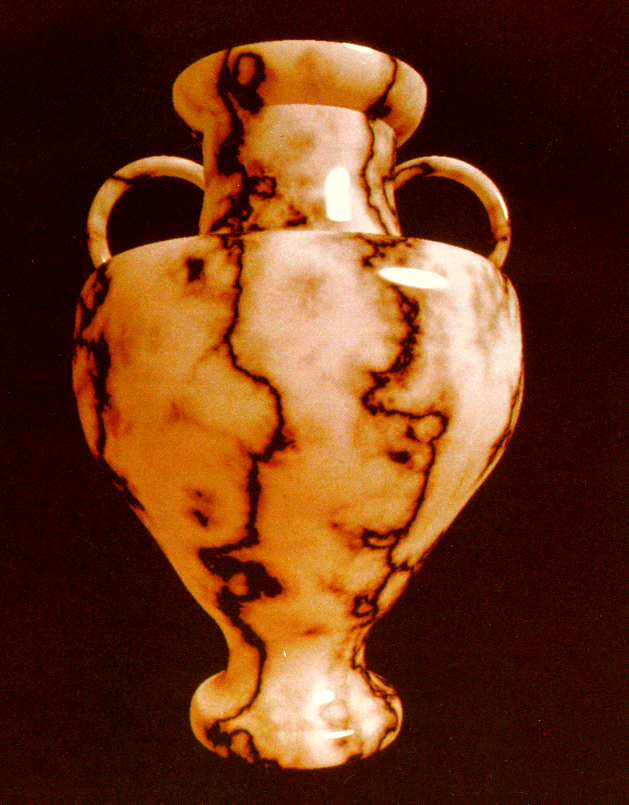
\includegraphics[scale=0.3]{obrazky-figures/PerlinNoiseVase.png}
	\caption{Váza s vygenerovanou texturou pomocí Perlinova šumu. Obrázek převzat z \cite{PerlinKen}}
	\label{PerlinVase}
\end{figure}

\subsubsection{Lepší gradientový šum}
Modifikovaná hashovací funkce kombinovaná s oddělenou gradientní tabulkou vylepšuje axialní dekorelaci. Jiné rekonstrukční jádro zlepšuje omezení pásma. Metoda projekce zlepšuje kvalitu šumu na 2D površích pomocí pevného šumu. Je třeba poznamenat, že tyto zlepšení platí pro několik druhů gradientových šumů mřížky. \cite{Kensler2008}

\subsubsection{Hardwarové implementace}
Již mnoho autorů představilo hardwarové implementace funkcí podobných Perlinovu šumu. Hart a spol. \cite{hart1999antialiased} prezentovali VLSI hardwarovou implementaci Perlinova šumu. Dále byly prezentovány GPU implementace Perlinova šumu, jak od Harta \cite{hart01} tak i od Olano \cite{ola05}. Dále je Perlinův šum nedílnou součástí OpenGL Shading Language (GLSL).

\subsection{Explicitní šumy}
\label{ExplicitNoises}
\textit{Explicitní šumy} generují šum explicitním způsobem předzpracováním a ukládají ho. Doslovně vzato, explicitní šumy nejsou procedurální šumové funkce, ale i tak jsou velmi podstatné. Dva reprezentativní příklady jsou, \hyperref[WaveletNoise]{vlnkový šum} a \hyperref[AnisotropNoise]{anisotropní} šum \cite{Lagae10}.

\subsubsection{Vlnkový šum}
\label{WaveletNoise}
Poprvé představen autory Cook a DeRose roku 2005 \cite{Cook05}. Perlinův šum ve větších vzdálenostech mívá problém s aliasingem a ztrátou detailů, z důvodu slabého pásmového omezení, kvůli tomu byla představena nová šumová funkce, která je téměř perfektně pásmově omezená.

Podstata algoritmu spočívá v následujících čtyřech krocích, které jsou vyobrazeny na obrázku \ref{fig:WaveletNoise}:

\begin{enumerate}
	\item Vytvoření obrazu $R$ vyplněného náhodným šumem.
	\item Snížení vzorkovací frekvence $R$ za účelem vytvoření obrazu o poloviční velikosti $R^\downarrow$.
	\item Zvětšení $R^\downarrow$ na plnou velikost $R^{\downarrow\uparrow}$.
	\item Odečtení $R^{\downarrow\uparrow}$ od originálního obrazu $R$ aby byl vytvořen výsledný obraz $N$.
\end{enumerate}

\begin{figure}[H]
	\centering
	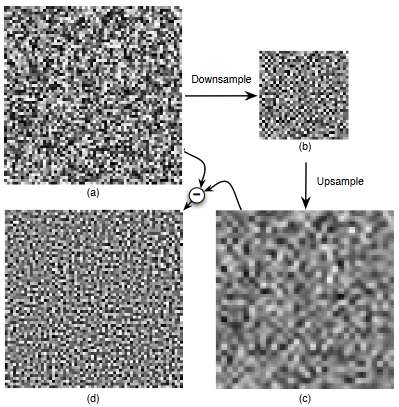
\includegraphics[scale=0.9]{obrazky-figures/WaveletNoise.png}
	\caption{Proces generování šumu.(a) Obrázek $R$ náhodného šumu, (b) o polovinu menší obrázek $R\downarrow$, (c) poloviční rozlišení obrázku $R{\downarrow\uparrow}$, (d) obraz pásmového šumu $N = R-R{\downarrow\uparrow}$. Obrázek převzat z \cite{Cook05}}
	\label{fig:WaveletNoise}
\end{figure}

Koeficienty šumu v dlaždici N jsou tedy vytvořeny z R a odstraněním části, která je reprezentovatelná na poloviční velikosti. Zbývá část, která není reprezentovatelná na poloviční velikosti, tj. pásmově omezená část. Filtry použité v krocích vzorkování dolů a nahoru jsou získány pomocí vlnkové analýzy. Rozšíření na více dimenzí je přímé.

\subsubsection{Anisotropní šum}
\label{AnisotropNoise}
Roku 2008, představil Goldberg a spol. \textit{anisotropní šum} \cite{Goldberg08}. Goldberg vypozoroval že existující šumové funkce podporují pouze isotropní filtrování, na což se také vztahuje aliasing a ztráta detailů, a představil novou funkci, která podporuje anisotropní filtrování na vysoké úrovni.

Hlavní myšlenkou bylo vygenerovat šumové textury tak, že frekvenční obor je rozdělen do orientovaných pod-pásem. Anizotropní šumové pásma mají nejen určitý rozsah škály, ve kterém jsou účinné, ale také mají preferovanou směrovou orientaci. Konstrukce takového šumu je založena na ovladatelných filtrech, které rozdělují frekvenční obor. Poskytují řadu vlastností, které jsou zásadní pro generování šumu:
\begin{enumerate}
	\item Každý filtr definuje pod-pásmo které je úzce lokalizované velikostí a orientací.
	\item Filtry implementují invertibilní transformaci. To znamená, že lze přesně obnovit signál z jeho dekompozice do pod-pásem.
	\item Filtry disponují možností točení orientace. Hlavním účelem je, že lineární interpolace filtrů může generovat filtr s přesně stejným profilem, ale s prostřední orientací.
\end{enumerate}

\begin{figure}[H]
	\centering
	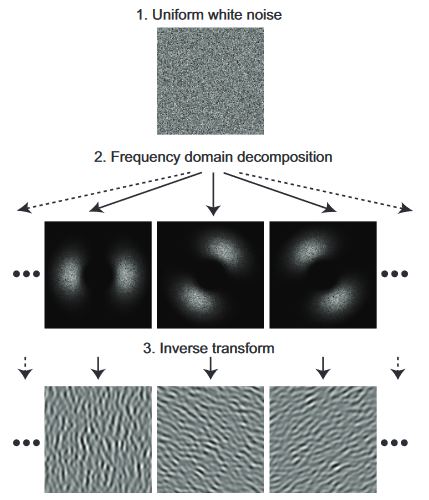
\includegraphics[scale=0.8]{obrazky-figures/AnisotropicNoise.png}
	\caption{Ilustrace spektrálního generování šumu. Dekompozice frekvenční domény má tři orientace. Jsou vidět tři orientované pod-pásma se stejnou velikostí a odpovídajícími obrazy prostorových domén, které se následně ukládají jako textury. Obrázek převzat z \cite{Goldberg08}.}
	\label{fig:AnisotropicNoise}
\end{figure}

Každý orientovaný pod-pásmový obraz je zabalen do jednoho kanálu 32bitového RGBA obrazu, což vede ke čtyřem orientacím na každou texturu. Obvykle použití čtyř nebo osmi pásů, tj. jedné nebo dvou textur, představuje dobrý kompromis mezi úložným prostorem, rychlostí vykreslování a kvalitou obrazu. Pod-pásma šumu jsou vypočítána dopředu pouze na jedné škále najednou. Všechny ostatní škály jsou generovány za běhu, jednoduše pomocí stupňování předem vypočítaných textur. \cite{Lagae10}

\subsubsection{Stochastické poddělení}
Fournier a spol. \cite{Fournier98}, který představil metodu středního posunu, uvedl také stochastický algoritmus dělení, pro generování přírodních nepravidelných fraktálních objektů a jevů, jako je terén. Lewis \cite{Lewis86,Lewis87} předvedl zobecněné stochastické poddělení, a generalizoval Fournierovu práci na libovolné autokorelační funkce.

\subsubsection{Fourierova spektrální syntéza}
\label{Fourier}
\textit{Fourierova spektrální syntéza} generuje šum s konkrétním výkonovým spektrem filtrováním bílého šumu ve frekvenční oblasti. Fourierova spektrální syntéza byla uvedena v počítačové grafice autorem Anjyo \cite{Anjyo88} Saupe a Voss \cite{Saupe1988}, kteří ji využili, aby vygenerovali náhodné fraktály a simulovaly přírodní jevy. Fourierova spektrální syntéza může být užitečná i při generování referenčních řešení pro šumové funkce, u kterých je známé očekávané výkonové spektrum.

\subsection{Řídké konvoluční šumy}
\label{SparseNoises}
\textit{Řídké konvoluční šumy} generují šum jako sumu náhodně pozicovaných a vážených kernelů. Třemi reprezentativními příklady jsou šum řídké konvoluce, \hyperref[SpotNoise]{bodový šum} a \hyperref[GaborNoise]{Gaborův šum}.

\subsubsection{Definice}
V sérii prací mezi lety 1984 a 1989 Lewis představil \textit{řídký konvoluční šum} \cite{Lewis84, Lewis86, Lewis89}.

Konstrukce řídkého konvolučního šumu je jednoduchá: libovolné jádro $k$ je konvoluváno se šumem Poissonova procesu $\gamma$.

\[N(x,y) = \int\gamma(u,v)k(x-u,y-v)dudv\]

Poissonův proces sestává z impulsů nekorelovaných intenzit $a_k$ situovaných na náhodných nezávisle na sobě zvolených pozicích $(x_k,y_k)$.

\[\gamma(x,y) = \sum_k a_k \delta(x-x_k,y-y_k)\]

Poissonův proces je řídký, což znamená že nedefinuje každý pixel nebo bod v prostoru, od toho je odvozený název \textit{řídká konvoluce}. Tento způsob použití řídkého impulsního šumu umožňuje alespoň nějakou výpočetní efektivitu, vzhledem k tomu že konvoluce efektivně rozprostírá jádro se škálou amplitudy pouze na určitých místech $(x_k, y_k)$.

Abychom vyhodnotili šum v konkrétním bodě, je nutné použít pouze jádra, která se s tímto bodem překrývají. Toto je urychleno zavedením virtuální mřížky, kde velikost buňky mřížky odpovídá poloměru jádra. Vyhodnocením pak zahrnuje pouze jádra, která jsou umístěna v buňce obsahující daný bod a těch v sousedních buňkách. Souřadnice buňky jsou také použity k zasazení generátoru náhodných čísel pro generování Poissonových impulzů umístěných v této buňce. Více podrobností a vylepšených schémat pro tento krok jsou uvedeny u Worleyho \cite{worley1996} a Lagae a spol. \cite{Lagae09}. I když Lewis \cite{Lewis89} popisuje několik optimalizací, jako je ukládání konstruovaných Poissonových impulzů za předpokladu koherentního přístupu, je řídká konvoluční metoda trochu pomalejší než jedna oktáva Perlinova šumu.

\begin{figure}[H]
	\centering
	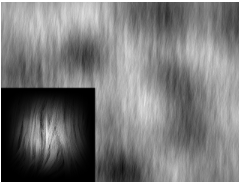
\includegraphics[scale=1]{obrazky-figures/SparseConvolutionNoise.png}
	\caption{\textit{Řídký konvoluční šum}. Vlevo dole: Vzorek obrázku vlasů. Vpravo: přibližná textura vlasů vytvořená pomoc9 2D řídké konvoluce. Obrázek převzat z \cite{Lagae10}.}
	\label{fig:SparseConvolutionNoise}
\end{figure}

Jelikož výkonové spektrum výstupu konvoluce je součinem vstupů a výkonové spektrum Poissonova impulsu je konstantní, je jednoduše škálovanou verzí tohoto jádra.

\subsubsection{Bodový šum}
\label{SpotNoise}
Jedná se o metodu generování stochastických textur pro vizualizaci skalárních a vektorových polí nad plochami. Na bodový šum lze nahlížet jako na explicitní formu řídkého konvolučního šumu, vypočítaného konverzí bodů, nebo Fourierovou spektrální syntézou (popsána v sekci \ref{Fourier}).

Van Wijk \cite{Wijk91} diskutuje vztah mezi bodem a texturou v detailech. Poukázal na několik důležitých konceptů, které později uvedl v kontextu šumu. Například, mapování textur na parametrických plochách, syntézu textur nad zakřivenými plochami jako alternativu pevnému šumu, a lokální kontrolu variací bodu. Dále lze pracovat s tvary, ostrostí hran, nebo různými vzory.

\begin{figure}[H]
	\centering
	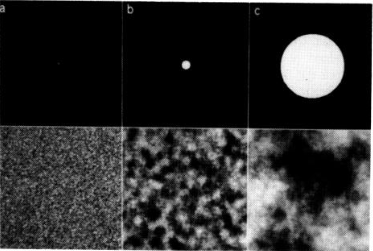
\includegraphics[scale=0.7]{obrazky-figures/SpotNoiseSize.png}
	\caption{Vztah mezi texturou a bodem. Na třech dvojicích obrázků jsou vidět tři různé velikosti bodu a tři různé šumy které se k těmto bodům vztahují. Obrázek převzat z \cite{Wijk91}.}
	\label{fig:SpotNoise}
\end{figure}
\begin{figure}[H]
	\centering
	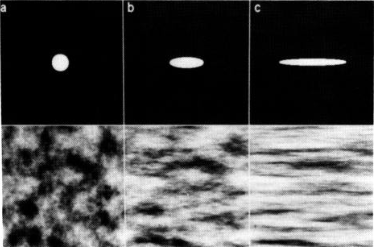
\includegraphics[scale=0.7]{obrazky-figures/SpotNoiseNonProportional.png}
	\caption{Na třech dvojicích obrázků je vidět jak se textury mění, když se velikost obrázku mění ne-proporcionálně. Obrázek převzat z \cite{Wijk91}.}
	\label{fig:SpotNoiseNonProportional}
\end{figure}

\subsubsection{Gaborův šum}
\label{GaborNoise}


\section{Výškové mapy}
\label{heightMaps}
Výškové mapy představují dvoudimenzionální mřížky obsahující výškové hodnoty, jež jsou častým prvkem v modelování terénu. Tyto mapy se běžně využívají jako klíčový prvek pro reprezentaci základu terénu v herním průmyslu. Pro tvorbu výškových map existuje mnoho algoritmů. Na obrázku \ref{HeightMap} je jednoduchá ukázka jak jednotlivé body na mapě mají hodnoty, podle kterých se dále určí jejich elevace. \cite{heightMap08}

Jedny z nejstarších algoritmů jsou metody založené na pododdělení. Segmenty v rámci vygenerované hrubé výškové mapy jsou iterativně rozdělovány, kde každá iterace navíc používá kontrolovanou náhodnost k přidávání detailů. Miller \cite{MillerRendering} popisuje některé varianty všeobecně známé metody středového posunu, ve které se výška nového bodu nastavuje na průměr hodnot jeho rohů v trojúhelníkovém nebo diamantovém tvaru, k němuž je přidán náhodný offset. Každou iterací se rozsah náhodných hodnot offsetu snižuje, podle parametru, který kontroluje hrubost výsledné výškové mapy. 

Generování výškových map se v dnešní době provádí převážně pomocí fraktálních generátorů šumu, jako je \hyperref[perlinNoise]{Perlinův šum}, který provádí generování šumu vzorkováním a interpolací bodů na mřížce náhodných vektorů.

Výškové mapy se mohou dále transformovat na základě běžných filtrací obrazu, například vyhlazování (smoothing), nebo simulací fyzikálních jevů, např. eroze. \cite{inproceedings}

\begin{figure}[H]
	\centering
	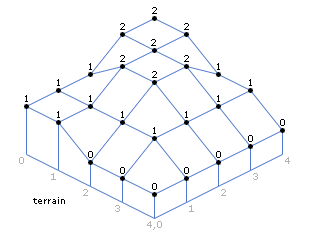
\includegraphics[scale=0.9]{obrazky-figures/HeightMap.png}
	\caption{Ukázka hodnot a jejich výšek výškových map}
	\label{HeightMap}
\end{figure}

Jednou z hlavních nevýhod výškových map je, že nepodporují tvorbu skalních převisů a jeskyní. Gamito a Musgrave \cite{Gamito2001ProceduralLW} navrhovali systém deformace terénu, který má za výsledek pravidelné, uměle vytvořené skalní převisy. O něco novější metoda \cite{Peytavie09} přináší propracovanější struktury s rozdílnými vrstvami materiálů, které podporují kameny, klenby, převisy a jeskyně. Příklady takto vygenerovaných struktur jsou vidět na obrázcích. \ref{PeytavieGen}

\begin{figure}[H]
	\centering
	\begin{subfigure}{0.475\textwidth}
		\centering
		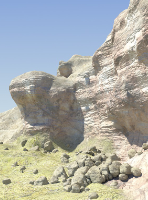
\includegraphics[scale=1]{obrazky-figures/Overhang.png}
		\caption{Vygenerované převisy}
	\end{subfigure}
	\begin{subfigure}{0.475\textwidth}
		\centering
		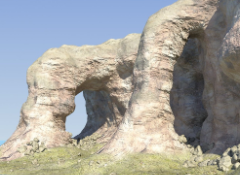
\includegraphics[scale=1]{obrazky-figures/Arches.png}
		\caption{Vygenerované kamenné klenby}
	\end{subfigure}
	\caption{Na obrázcích jsou vidět klenby a převisy vygenerované pomocí algoritmu vytvořeného Peytaviem, obrázky jsou převzaty z \cite{Peytavie09}}
	\label{PeytavieGen}
\end{figure}

\chapter{Procedurální generování krajiny}
\label{terrain}
Procedurální generování krajiny se řadí ke složitějším tématům PG. Je tomu tak hlavně kvůli tomu, že se k tomuto typu generování většinou používají výškové mapy (height maps), podle kterých se ohodnocují jednotlivé pixely, jak je popsáno v sekci \ref{heightMaps}. Jakmile jsou všechny pixely ohodnoceny, jsou tři různé způsoby jak postupovat:
\begin{itemize}
	\item ruční vykreslování textur,
	\item aplikování textur na ručně vytvořené regiony podle výšky,
	\item vygenerování textur po analyzování výšek na vygenerované výškové mapě.
\end{itemize}
První metoda je výhodná v tom, že textury ručně vykreslené lze udělat na míru a žádný algoritmus je nemůže replikovat. Bohužel jsou časově náročné a jejich kvalita přímo závisí na schopnostech výtvarníka.

Druhá metoda je podobná, nakreslí se barvy na určitá místa, kam si designer myslí že by se mohly hodit hory, řeky, nebo země. Jedná se o docela obvyklou metodu, která přináší velice kvalitní výsledky, ale stále se jedná o manuální techniku.

Třetí metoda používá data height mapy a vypočítává jakou texturu použít na které místo. Nízké hodnoty (tmavší místa) se používají například jako oceány, střední hodnoty se vyhodnocují jako země/tráva a na vysoké hodnoty (světlá místa) se nanášejí textury hor nebo kamení. Při generování ve 3D hrách lze ještě započítávat takzvané sklony (slopes), díky kterým je možné oddělovat vyšší plochy od nižších pomocí dalších textur například kamene. Tato metoda je více rozvedena v sekci \ref{heightMaps}.

Vzhledem k tomu že první dva postupy vyžadují mechanické vykreslování buď barvy, nebo textur on designéra, nedá se o nich mluvit jako o čistě procedurálních metodách. Naopak postup třetí tomuto popisu zcela odpovídá, neboť kompletně závisí na height mapě a není nutná žádná akce návrháře \cite{madoc59000}.

\paragraph*{Generování oblastí lze rozdělit následovně:}
\begin{description}
	\item[Vytváření půdorysu] Zahrnuje vytvoření země, moří, řek, hor, atd. Všechny tyto oblasti jsou otevřeného typu. Také můžeme rozumět pod generováním půdorysu i vytváření uzavřeného typu oblastí, například rozložení jednotlivých místností jeskynního komplexu, vytvoření bludiště a jeho cest. 
	
	\item[Přidání vegetace a objektů] Tento bod v podstatě navazuje na předchozí, je potřeba abychom měli vytvořený půdorys, aby bylo kam přidávat a rozmísťovat další objekty. Jedná se o bod do kterého spadá vegetace, budovy, atd. Programu se zadávají různá omezení na množství vegetace, místa kam který objekt lze přidávat a další omezení.
\end{description} 

\begin{figure}[h]
	\centering
	\begin{subfigure}{0.475\textwidth}
		\centering
		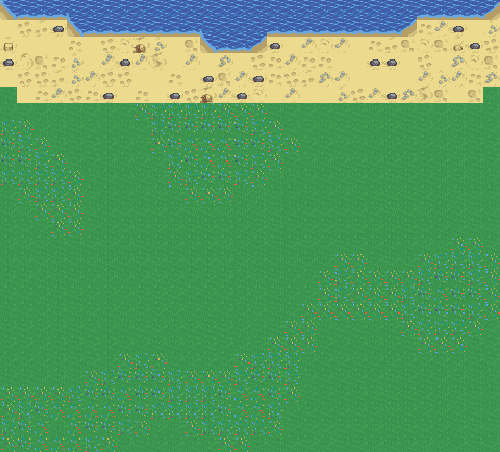
\includegraphics[scale=0.5]{obrazky-figures/layoutNoTrees.png}
		\caption{Vygenerovaný půdorys oblasti}
	\end{subfigure}
	\begin{subfigure}{0.475\textwidth}
		\centering
		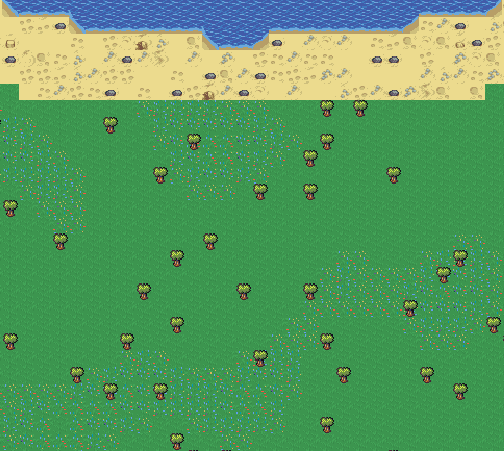
\includegraphics[scale=0.5]{obrazky-figures/treesAdded.png}
		\caption{Přidané stromy k půdorysu}
	\end{subfigure}
	\caption{Na obrázcích jsou vidět různé postupy generování obsahu z této hry, na obrázku a je vygenerovaný půdorys oblasti i s mořem a pláží, na obrázku b se k tomu přidaly stromy}
\end{figure}

\iffalse

\section{Metody pro procedurální generování krajiny}
Tato část se zabývá průzkumem procedurálních metod, aplikovaných na modelování terénu. Pojednává o důležitých aspektech, jako je realističnost výstupu, náročnost algoritmu a prostředky pomocí kterých je uživatel schopen ovlivnit a kontrolovat proces generování.~\cite{inproceedings}

\subsubsection{Porovnání metod}
\todo{porovnání jednotlivých metod}

\includegraphics[scale=0.3]{obrazky-figures/keep-calm.png}

\fi

\chapter{Návrh řešení}
\label{solution}
Tato kapitola popisuje vybrané technologie, které byly použity k vývoji hry a z jakého důvodu, zvolené metody jak budou procedurální mapy vytvářeny, návrhy algoritmů a způsobů generování oblastí. 

\section{Vybrané technologie}
V mé práci jsem se rozhodl pro použití herního enginu Unity, který je podrobněji popsán v sekci \ref{unity}. Před samotným začátkem práce jsem zhodnotil, že vývojové prostředí Unity nabízí mnoho výhod a pro vývoj procedurálního generování a následné hry bude ideální.

Dalším z důvodů pro volbu Unity je jazyk C\#, který nabízí mnoho knihoven, které budou užitečné při tvorbě hry. Plusem je že C\# disponuje silnou typovou kontrolou, což znamená, že chyby v kódu jsou odhaleny během překladu, což usnadňuje odhalování a opravování chyb při vývoji.

C\# nabízí širokou škálu knihoven, ale tou pro mě nejdůležitější byla knihovna Mathf, která kromě mnoha matematických funkcí obsahuje také funkci Perlinova šumu. Jazyk C\# je obecně velmi užívaný a tím pádem má i velkou aktivní komunitu vývojářů, přispívajících do knihoven, nástrojů, frameworků, poskytují podporu a návody, které pomáhají ostatním vývojářům efektivně pracovat s procedurálním generováním. 

Některé další výhody použití programovacího jazyka C\# v kombinaci s Unity pro tvorbu her s procedurálním generováním zahrnují:

\begin{enumerate}
	\item \textbf{Snadná integrace s Unity:} C\# je primárním programovacím jazykem pro vývoj her v Unity, což znamená že má těsnou integraci s Unity API a prostředím.
	\item \textbf{Objektově orientovaný přístup:} C\# je objektově orientovaný jazyk, což umožňuje vytvářet modulární a znovupoužitelný kód. To usnadňuje organizaci a správu algoritmů a umožňuje snadnou rozšiřitelnost, údržbu a znovupoužitelnost v jiných projektech.
	\item \textbf{Platformní nezávislost:} Díky tomu, že Unity podporuje mnoho různých platforem, může být C\# kód psaný v Unity použit na vytváření her pro různé platformy, včetně mobilních zařízení, stolních počítačů, konzolí a webu, což zvyšuje dostupnost a dosah hry.
\end{enumerate}

Vývojovým prostředím jsem zvolil Visual Studio, které je primárním IDE doporučované společností Unity pro vývoj v jazyce C\#. Poskytuje silnou integraci s Unity Editorem, což znamená, že lze snadno vytvářet a upravovat skripty přímo v rámci Unity Editoru. Existuje ale několik dalších důvodů, proč zvolit Visual Studio jako vývojové prostředí:
 
\begin{enumerate}
	\item \textbf{Široká podpora a komunita:} Visual Studio je velmi populární vývojové prostředí s rozsáhlou komunitou uživatelů a dostupností online dokumentace a návodů. To je užitečné pro získání podpory a řešení problémů během vývoje.
	\item \textbf{Pokročilé funkce pro vývoj:} Nabízí mnoho pokročilých funkcí pro vývoj v jazyce C\#, jako je inteligentní vyplňování kódu, refactoring, ladění za běhu a integrace s verzovacími systémy. 
	\item \textbf{Podpora pro rozšíření:} Visual Studio umožňuje rozšiřování funkcí pomocí různých rozšíření, balíčků a doplňků, která mohou usnadni proces vývoje a zvýšit produktivitu.
\end{enumerate}

\section{Návrh procedurálního generování oblastí}
V této sekci je popsán způsob jakým se generují jednotlivé oblasti, použité algoritmy, metody a různé úpravy pomocí kterých bude vytvořena 2D mapa, na které se následně bude odehrávat samotná hra, jejíž návrh je detailněji popsán v sekci \ref{GameDesign}.

\subsection{Zvolený šum}
Pro generování samotného šumu jsem vybral známý Perlinův šum, detailně popsán v sekci \ref{perlinNoise}, který je relativně jednoduchý na implementaci a jeho porozumění. Algoritmus kterým je implementován je intuitivní a snadno přenositelný do různých herních prostředí. Zde je pár dalších důvodů proč jsem vybral právě Perlinův šum pro generování:

\begin{description}
	\item[Hladkost a přirozenost] Perlinův šum poskytuje hladké a přirozené výsledky. Jeho charakteristika umožňuje vytvářet organické a realistické terény.
	\item[Efektivita] Perlinův šum je poměrně efektivní z hlediska výpočetní náročnosti. Jeho algoritmus umožňuje generování šumu s rozumným výkonem a nízkou paměťovou náročností.
\end{description}

Oproti například vlnkovému šumu, sekce \ref{WaveletNoise}, sice nemá takovou flexibilitu v nastavení detailů a škálování, ale kvůli přirozenosti jsem se rozhodl pro Perlinův. Perlinův šum bude mít mnoho vlastností, detailně popsány v sekci implementace \ref{PerlinNoiseImplement}, ale asi nejdůležitější bude vlastnost \textit{seed}, pomocí které bude možné kteroukoliv mapu znovu vygenerovat.

\subsection{Algoritmus procedurálního generování mapy}
Procedurální generování mapy je jedním z hlavních cílů této práce. Pro generování samotné mapy, se bude využívat již zmíněný Perlinův šum, s použitím výškových map, popsány v sekci \ref{heightMaps}. Každá oblast, země, voda, skály, nebo pláže, bude mít definovaný rozsah výšky na výškové mapě. Unity disponuje nástrojem zvaným \textit{tilemap}, jedná se o čtvercovou mřížku, do jejíž buněk lze skládat takzvané \textit{tiles} (dlaždice). Velkou výhodou těchto tilemap je, že každý bod reprezentuje jeden tile, tím pádem po ohodnocení bodu lze pouze položit odpovídající tile.

\begin{figure}[H]
	\centering
	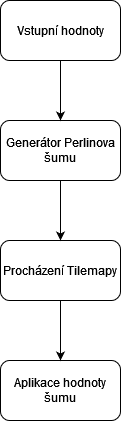
\includegraphics[scale=0.9]{obrazky-figures/AlgoritmusDiagram.png}
	\caption{Ilustrace navrhovaného diagramu algoritmu, který bude generovat mapu}
	\label{AlgoritmusDiagram}
\end{figure}

Kvůli jednodušší a srozumitelné interakci s uživatelem při generování map v Unity, navrhuji skript, obsahující následující algoritmus, vyobrazený na obrázku \ref{AlgoritmusDiagram}:

\begin{description}
	\item[Vstupní hodnoty] Uživatel zadá potřebné hodnoty pro generování šumu, jako jsou výška a šířka mapy a přiblížení šumu. Tyto hodnoty určují vlastnosti výsledného šumu a tím i vzhled herního terénu.
	\item[Generátor Perlinova šumu] Na základě zadaných parametrů se generuje dvoudimenzionální Perlinův šum. Tento šum je vytvořen pomocí algoritmu Perlinova šumu, který produkuje hladké a přirozeně vypadající přechody mezi různými hodnotami.
	\item[Procházení tilemapy] Procházením každého bodu na tilemapě se určí, jaký typ terénu nebo objekty by měl být umístěn na daném místě. To se prování porovnáním hodnoty Perlinova šumu v daném bodě s definovanými prahovými hodnotami nebo regiony.
	\item[Aplikace hodnoty šumu] Na základě porovnání s definovaným regiony se do každého bodu na tilemapě vloží odpovídající tile, který reprezentuje určitý typ terénu, jako jsou travnaté plochy, hory, jezera nebo lesy. Díky tomu může být vytvořen pestrobarevný a realistický herní svět.
\end{description}

Tento algoritmus poskytuje uživatelům možnost tvořit rozmanitá a realistická herní prostředí v Unity pomocí Perlinova šumu a tilemap. Samotný algoritmus je navržen tak, aby poskytoval co největší kontrolu na vzhledem vygenerovaných map. Díky flexibilitě a jednoduchosti tohoto přístupu může být proces tvorby herního světa intuitivní a rychlý. 

\section{Návrh hry}
\label{GameDesign}
Tato sekce popisuje žánr, styl, cíle a ovládání samotné hry, založené na procedurálním generování 2D map v herním prostředí.

Hra bude kombinovat prvky real-time strategie (RTS) s prvky survival žánru, vyžaduje strategické plánování a rychlé rozhodování v rámci nepřetržitého boje o přežití. Cílem hry je bránit se pravidelným nájezdům nepřátel, zatímco hráč současně buduje a rozvíjí svoji obranou sílu.

Při výběru hratelné rasy a dvou začínajících postav na začátku hry hráči rozhodují o strategickém směru, kterým se jejich osada bude ubírat. Různé rasy mohou poskytovat specifické výhody a jedinečné schopnosti, což ovlivňuje strategii budování a obrany hráčů.

Kromě budování základní infrastruktury, jako jsou farmy pro zajištění potravin, musí hráči také efektivně využívat dostupné prostředky a suroviny k budování různých typů obranných struktur. To může zahrnovat stavbu opevněných hradeb, věží, pastí, které mají za cíl zpomalit nebo zastavit postup nepřátelských sil.

Kromě obrany před nepřáteli se hráči budou muset vypořádat s dalšími přírodními a lidskými hrozbami, jako je nedostatek surovin, nebo náhlé změny počasí.

Vývoj ve hře je doprovázen možností rozšíření a vylepšení stávajících budov, což umožňuje vybudovat silnější a odolnější obranné systémy. Zároveň se hráči musí adaptovat na nové výzvy a nepředvídatelné situace.

\subsection{Grafika}
Hra je navržena jako 2D hra s pohledem zhora (top-down), což poskytne hráčům přehledný pohled na herní prostředí a umožní jim snadnou navigaci a řízení svých jednotek. Grafický styl hry bude pixelový, s použitím převážně 16x16 pixelových spriteů. Tento styl grafiky je známý svou jednoduchostí. Modelů tohoto stylu je mnoho volně dostupných a v případě potřeby lze bez problémů dotvořit vlastní. Díky tomuto stylu grafiky bude zároveň možné udržet nízké nároky na hardwarové prostředky, což umožní hladký běh hry i na starších zařízeních.

\subsection{Jednoduchá umělá inteligence nepřátel}
Umělá inteligence nepřátel bude implementována pomocí skriptů, které budou mít za úkol detekovat hráče v okolí a podle toho reagovat, včetně pronásledování a útoku na hráče. Pro pohyb po mapě bude využit vestavěný systém v Unity nazývaný NavMesh. Každá jednotka, která se má pohybovat po mapě, bude mít přiděleného NavMesh agenta, který bude schopen reagovat na podloží definované NavMesh surface. Tímto způsobem bude umožněno nepřátelským jednotkám plánovat svůj pohyb po herním světě s ohledem na dostupné průchody a neprůchodné oblasti definované v NavMesh surface, což vytvoří realističtější a dynamické chování nepřátel.

\subsection{NavMesh funkcionalita}
NavMesh je vestavěný systém v Unity, který umožňuje jednotkám v herním světě plánovat svůj pohyb a navigovat přes prostředí. Jedná se o komplexní nástroj pro tvorbu navigačních dat, která definují, kde se mohou jednotky pohybovat a kudy nemohou.

NavMesh systém v Unity funguje následovně:

\begin{enumerate}
	\item Nejprve je třeba vytvořit navigační síť v herním světě. To se obvykle provádí pomocí generování NavMesh surface, které automaticky vytvoří navigační data podle geometrie herního světa.
	\item Poté co je NavMesh vytvořen, mohou být jednotkám přiděleni NavMesh agenti. Jedná se o komponentu umožňující jednotkám navigaci přes NavMesh a plánovat jejich pohyb.
	\item Agenti mohou plánovat svůj pohyb v reálném čase na základě polohy jednotky a cíle, kam se má jednotka dostat. NavMesh agenti automaticky vyhledají nejkratší cestu k danému cíli.
	\item NavMesh může být dynamicky aktualizován v průběhu hry, což umožňuje jednotkám reagovat na změny v prostředí a dynamicky plánovat svůj pohyb.
\end{enumerate}

\subsection{Ekonomika hry}
Hra bude obsahovat základní suroviny jako je dřevo, kámen a jídlo, které budou hrát klíčovou roli v průběhu hry.

\begin{description}
	\item[Dřevo:] Dřevo lze získat těžbou stromů, které budou rozmístěné po herní mapě. Dřevo bude nezbytné pro výstavbu obranných struktur a budování celé osady. Jeho nedostatek může ztížit možnosti obrany a rozvoje osady.
	\item[Kámen:] Kámen lze získat kopáním skal a hornin v okolí herního prostředí. Bude sloužit jako stavební a vylepšující materiál pro obranné struktury a osadu. Nedostatek kamene může omezit hráčovy možnosti vylepšení obrany.
	\item[Jídlo:] Jídlo bude nezbytné pro přežití obyvatel osady. Hráči budou moci získat jídlo pomocí farmaření, kde budou pěstovat plodiny, nebo lovením divoké zvěře. Nedostatek jídla může vést k hladovění osadníků a jejich úmrtí, což může znamenat prohru.
\end{description}

Všechny tyto suroviny budou hrát klíčovou roli v ekonomice a strategii hry. Hráči budou muset efektivně spravovat jejich zdroje a využívat je pro zajištění bezpečnosti a přežití své osady.

\todo{Blbost>>?}

\subsection{Model dat}
Při návrhu modelu dat jsem vycházel z potřeb herního prostředí a funkcí, která hra poskytuje. Model dat je navržen tak, aby reflektoval vztahy mezi jednotlivými herními entitami a umožňoval efektivní správu a manipulaci s daty během hry. Hlavními entitami v modelu dat jsou postavy, objekty, suroviny a herní události.

Postavy jsou reprezentovány jako objekty s atributy jako jméno, životy, úroveň atd. Objekty jsou rozděleny do kategorií jako budovy, překážky atd. Suroviny jsou reprezentovány jako objekty s atributy jako typ suroviny a množství.

Vztahy mezi entitami jsou definovány pomocí vazeb a asociací, což umožňuje přesné modelování herních mechanismů a interakcí. Například postava může vlastnit určité objekty, suroviny mohou být sbírány a využívány k výrobě dalších objektů a herní události mohou ovlivňovat stav postav a objektů.

\subsubsection{ER diagram:}
Pro lepší představu modelu dat je zde uveden ER diagram, což je grafický nástroj používaný k vizualizaci a popisu struktury datového modelu.

\todo{diagram dodělat}


\chapter{Implementace}
\label{implementace}
Tato část se věnuje podrobnostem implementace skriptů, jež jsou klíčovými součástmi vytváření finální hry a struktury samotného projektu.

\section{Architektura hry}
V této sekci se zabývám popisem architektury samotného projektu a jeho struktury. Dále je zde ER diagram popisující vztah jednotlivých datových struktur.

\subsection{Struktura projektu}
Jednotlivé části projektu obsahují klíčové prvky této práce a jsou následovně rozděleny do jednotlivých složek. Tato sekce popisuje hlavní složky do kterých je tento projekt rozdělen.

\todo{přidat diagram struktury složek}

\begin{description}
	\item[Animations] Tato složka obsahuje soubory s animacemi postav a okolí ve hře. Animace jsou klíčovým prvkem pro pohyb a vizuální efekty herních postav a prostředí. V této složce se nachází více dalších podsložek které dále rozdělují animace tak, aby usnadňovaly snadný přístup a správu animačních souborů.
	\item[Graphics] Ve složceGraphics se nacházejí všechny grafické podklady použité v této hře, jako jsou textury, sprity, modely a další vizuální prvky. Grafické podklady jsou důležité pro vytváření vizuálního prostředí této hry a přispívají k celkovému vzhledu a atmosféře.
	\item[Prefabs] Prefabs jsou předvytvořené herní objekty s přiřazenými skripty a dalšími vlastnostmi, které lze opakovaně využívat ve hře.
	
	Tato složka obsahuje klíčové herní objekty, které jsou vytvořeny, konfigurovány předem a mohou být snadno použity v různých scénách hry. Příklad využití je například u stromů, které mají při inicializaci stejné vlastnosti a tak mají vlastní prefab, který tyto informace, společně se spritem, obsahuje.
	\item[Scenes] V této složce jsou definované herní scény, jako jsou menu, nebo samotná hlavní herní scéna hry. Každá scéna obsahuje specifické herní objekty, nastavení a logiku potřebnou pro danou část hry.
	\item[ScriptableObjects] ScriptableObjects jsou objekty vytvořené pomocí skriptů, které dědí z třídy ScriptableObject vestavěné v Unity. Tyto objekty mohou uchovávat data, nastavení a další informace, které lze použít v různých částech hry, hodí se například pro stavitelné objekty které budou mít vždy stejné základní vlastnosti, jako je sprite, název, nebo kategorii do které spadá, ke kterým si potom vývojář přidá potřebné skripty.
	\item[Scripts] Ve složce scripts se nacházejí všechny skripty potřebné k běhu hry. Skripty obsahují herní logiku, ovladače, umělou inteligenci, UI interakce a další funkce potřebné k implementaci funkcí a chování vaší hry. Tato složka je dále rozdělená do podsložek, z důvodu ještě lepší organizace, přístupu a správy skriptů
\end{description}

Při organizaci složek jsem zohlednil několik kritérií, která jsou důležitá pro efektivní správu a vývoj projektu. Při navrhování struktury složek jsem se zaměřil na funkční oddělení a jednoduchost formátu. Hlavní složky projektu jsou rozděleny podle typu obsahu a funkčnosti, co usnadňuje navigaci a správu projektu.

Dalším hlediskem na které jsem se zaměřil bylo oddělení logiky a dat, přičemž skripty obsahují herní logiku a funkce, zatímco ScriptableObjects slouží k uchování dat a nastavení, nezávislých na konkrétních instancích herních objektů. Toto rozdělení pomáhá udržovat kód čistý a přehledný, což usnadňuje údržbu a správu projektu v průběhu vývoje.

\section{Implementace algoritmů}
Tato sekce detailně popisuje implementaci jednotlivých algoritmů včetně příkladů kódu.

\subsection{Generování terénu}
Tato sekce se detailně zaměřuje na konkrétní implementaci Perlinova šumu v prostředí Unity pomocí skriptů v jazyce C\#. Vysvětluje postup krok za krokem a představuje klíčové prvky implementace jako je využití Perlinova šumu, detailně vysvětleného v sekci \ref{perlinNoise}, který je implementovaný v knihovně \textit{Mathf}. 

\subsubsection{Skript pro inicializaci a nastavení šumu}
Skriptem, který má za úkol inicializovat generátor Perlinova šumu a umožňuje nastavení klíčových parametrů, jako jsou šířka a výška mapy, seed, přiblížení šumu, oktávy, apod. pro dosažení různorodých terénů, je pojmenován \textit{MapGenerator.cs} \todo{bez .cs?}. 

Jedná se o skript který je přímo přiřazený hernímu objektu jménem \textit{Map Generator}, ve kterém může vývojář pohodlně zadávat potřebné hodnoty pro generování šumu a samotného terénu.

\begin{lstlisting}
using system;

public class MapGenerator : MonoBehaviour
{
	public int mapWidth;
	public int mapHeight;
	public float noiseScale;
	public int octaves;
	public int octaves;
	[Range(0f, 1f)]
	public float persistance;
	public float lacunarity;
	
	public int seed;
	public Vector2 offset;	
	
	public void GenerateMap()
	{
		.
		.
		.
		float[,] noiseMap = noise.GenerateNoiseMap(mapWidth, 
		mapHeight, seed, noiseScale, octaves, persistance, lacunarity, offset);
		.
		.
		.
	}
}
\end{lstlisting}
\iffalse
\section{Perlinův šum}
\label{PerlinNoiseImplement}
\textcolor{gray}{\blindtext[60]}
\chapter{Experimenty a vyhodnocení}
\label{experiments}
\section{testování}
\label{tests}
\textcolor{gray}{\blindtext[30]}

\chapter{Závěr}
\label{end}
\textcolor{gray}{\blindtext[4]}
\fi